\documentclass[9pt,twocolumn,twoside]{pnas-new}

\articletype{BIOLOGICAL SCIENCES}
\templatetype{pnasresearcharticle}
% Generated by scripts/build_paper_claim_ledger.py; do not edit by hand.
\providecommand{\PaperRoundingPolicy}{Four decimals for absolute metrics; two percentage points for development effects; three decimals for correlations and pair-level metrics.}
\providecommand{\AlignedMinusShiftedAUPRCLower}{0.1767}
\providecommand{\AlignedMinusShiftedAUPRCMedian}{0.1993}
\providecommand{\AlignedMinusShiftedAUPRCUpper}{0.2239}
\providecommand{\AlignedMinusShiftedAUROCLower}{0.1754}
\providecommand{\AlignedMinusShiftedAUROCMedian}{0.1926}
\providecommand{\AlignedMinusShiftedAUROCUpper}{0.2109}
\providecommand{\AlignedMinusShiftedFOneLower}{0.1155}
\providecommand{\AlignedMinusShiftedFOneMedian}{0.1311}
\providecommand{\AlignedMinusShiftedFOneUpper}{0.1477}
\providecommand{\AllADeltaAUPRCLower}{-0.0967}
\providecommand{\AllADeltaAUPRCMedian}{-0.0673}
\providecommand{\AllADeltaAUPRCUpper}{-0.0404}
\providecommand{\AllADeltaAUROCLower}{-0.0925}
\providecommand{\AllADeltaAUROCMedian}{-0.0664}
\providecommand{\AllADeltaAUROCUpper}{-0.0438}
\providecommand{\AllADeltaBrierLower}{0.0330}
\providecommand{\AllADeltaBrierMedian}{0.0497}
\providecommand{\AllADeltaBrierUpper}{0.0677}
\providecommand{\AllADeltaFOneLower}{-0.0878}
\providecommand{\AllADeltaFOneMedian}{-0.0599}
\providecommand{\AllADeltaFOneUpper}{-0.0365}
\providecommand{\ArteryADARProAUPRC}{0.9485}
\providecommand{\ArteryADARProAUROC}{0.9477}
\providecommand{\ArteryADARProBrier}{0.0879}
\providecommand{\ArteryADARProFOne}{0.8869}
\providecommand{\ArteryADARProPrecision}{0.8840}
\providecommand{\ArteryADARProRecall}{0.8899}
\providecommand{\ArteryADARProSpecificity}{0.8650}
\providecommand{\ArteryAdarEditAUPRC}{0.9262}
\providecommand{\ArteryAdarEditAUROC}{0.9238}
\providecommand{\ArteryAdarEditBrier}{0.1077}
\providecommand{\ArteryAdarEditFOne}{0.8671}
\providecommand{\ArteryAdarEditPrecision}{0.8345}
\providecommand{\ArteryAdarEditRecall}{0.9023}
\providecommand{\ArteryAdarEditSpecificity}{0.7930}
\providecommand{\ArteryDeltaAUPRC}{0.0224}
\providecommand{\ArteryDeltaAUROC}{0.0239}
\providecommand{\ArteryDeltaBrier}{-0.0198}
\providecommand{\ArteryDeltaFOne}{0.0199}
\providecommand{\ArteryDeltaPrecision}{0.0496}
\providecommand{\ArteryDeltaRecall}{-0.0125}
\providecommand{\ArteryDeltaSpecificity}{0.0720}
\providecommand{\ArteryEngagementCombinedGeometryAnyEditedAUROC}{0.816}
\providecommand{\ArteryEngagementCombinedGeometryRSquared}{0.270}
\providecommand{\ArteryEngagementCombinedGeometrySpearman}{0.536}
\providecommand{\ArteryEngagementGraphOnlyAnyEditedAUROC}{0.461}
\providecommand{\ArteryEngagementGraphOnlyRSquared}{0.053}
\providecommand{\ArteryEngagementGraphOnlySpearman}{0.203}
\providecommand{\ArteryFPRescueRate}{43.9}
\providecommand{\ArteryGapRho}{-0.482}
\providecommand{\ArteryMatchedRecallFPAvoided}{126}
\providecommand{\ArteryPairFirstAUPRCLower}{+0.79}
\providecommand{\ArteryPairFirstAUPRCMedian}{+1.37}
\providecommand{\ArteryPairFirstAUPRCUpper}{+1.97}
\providecommand{\ArteryPairFirstAUROCLower}{+0.80}
\providecommand{\ArteryPairFirstAUROCMedian}{+1.22}
\providecommand{\ArteryPairFirstAUROCUpper}{+1.66}
\providecommand{\ArteryPairFirstFOneLower}{+0.10}
\providecommand{\ArteryPairFirstFOneMedian}{+0.69}
\providecommand{\ArteryPairFirstFOneUpper}{+1.27}
\providecommand{\ArteryTPDamageRate}{4.9}
\providecommand{\BrainADARProAUPRC}{0.9504}
\providecommand{\BrainADARProAUROC}{0.9508}
\providecommand{\BrainADARProBrier}{0.0855}
\providecommand{\BrainADARProFOne}{0.8902}
\providecommand{\BrainADARProPrecision}{0.8741}
\providecommand{\BrainADARProRecall}{0.9069}
\providecommand{\BrainADARProSpecificity}{0.8529}
\providecommand{\BrainAdarEditAUPRC}{0.9286}
\providecommand{\BrainAdarEditAUROC}{0.9301}
\providecommand{\BrainAdarEditBrier}{0.1050}
\providecommand{\BrainAdarEditFOne}{0.8689}
\providecommand{\BrainAdarEditPrecision}{0.8371}
\providecommand{\BrainAdarEditRecall}{0.9032}
\providecommand{\BrainAdarEditSpecificity}{0.8021}
\providecommand{\BrainDeltaAUPRC}{0.0217}
\providecommand{\BrainDeltaAUROC}{0.0206}
\providecommand{\BrainDeltaBrier}{-0.0195}
\providecommand{\BrainDeltaFOne}{0.0213}
\providecommand{\BrainDeltaPrecision}{0.0370}
\providecommand{\BrainDeltaRecall}{0.0037}
\providecommand{\BrainDeltaSpecificity}{0.0507}
\providecommand{\BrainEngagementCombinedGeometryAnyEditedAUROC}{0.749}
\providecommand{\BrainEngagementCombinedGeometryRSquared}{0.239}
\providecommand{\BrainEngagementCombinedGeometrySpearman}{0.501}
\providecommand{\BrainEngagementGraphOnlyAnyEditedAUROC}{0.525}
\providecommand{\BrainEngagementGraphOnlyRSquared}{0.050}
\providecommand{\BrainEngagementGraphOnlySpearman}{0.218}
\providecommand{\BrainFPRescueRate}{38.6}
\providecommand{\BrainGapRho}{-0.425}
\providecommand{\BrainMatchedRecallFPAvoided}{119}
\providecommand{\BrainPairFirstAUPRCLower}{+1.02}
\providecommand{\BrainPairFirstAUPRCMedian}{+1.64}
\providecommand{\BrainPairFirstAUPRCUpper}{+2.20}
\providecommand{\BrainPairFirstAUROCLower}{+0.82}
\providecommand{\BrainPairFirstAUROCMedian}{+1.17}
\providecommand{\BrainPairFirstAUROCUpper}{+1.54}
\providecommand{\BrainPairFirstFOneLower}{+0.61}
\providecommand{\BrainPairFirstFOneMedian}{+1.11}
\providecommand{\BrainPairFirstFOneUpper}{+1.64}
\providecommand{\BrainTPDamageRate}{3.3}
\providecommand{\CombinedADARProAUPRC}{0.9513}
\providecommand{\CombinedADARProAUROC}{0.9491}
\providecommand{\CombinedADARProBrier}{0.0870}
\providecommand{\CombinedADARProFOne}{0.8852}
\providecommand{\CombinedADARProPrecision}{0.8463}
\providecommand{\CombinedADARProRecall}{0.9279}
\providecommand{\CombinedADARProSpecificity}{0.8159}
\providecommand{\CombinedAdarEditAUPRC}{0.9356}
\providecommand{\CombinedAdarEditAUROC}{0.9331}
\providecommand{\CombinedAdarEditBrier}{0.1043}
\providecommand{\CombinedAdarEditFOne}{0.8674}
\providecommand{\CombinedAdarEditPrecision}{0.8334}
\providecommand{\CombinedAdarEditRecall}{0.9043}
\providecommand{\CombinedAdarEditSpecificity}{0.8026}
\providecommand{\CombinedDeltaAUPRC}{0.0157}
\providecommand{\CombinedDeltaAUROC}{0.0160}
\providecommand{\CombinedDeltaBrier}{-0.0173}
\providecommand{\CombinedDeltaFOne}{0.0178}
\providecommand{\CombinedDeltaPrecision}{0.0129}
\providecommand{\CombinedDeltaRecall}{0.0236}
\providecommand{\CombinedDeltaSpecificity}{0.0133}
\providecommand{\CombinedFPRescueRate}{32.0}
\providecommand{\CombinedMatchedRecallFPAvoided}{148}
\providecommand{\CombinedPairFirstAUPRCLower}{+1.15}
\providecommand{\CombinedPairFirstAUPRCMedian}{+1.69}
\providecommand{\CombinedPairFirstAUPRCUpper}{+2.24}
\providecommand{\CombinedPairFirstAUROCLower}{+1.09}
\providecommand{\CombinedPairFirstAUROCMedian}{+1.45}
\providecommand{\CombinedPairFirstAUROCUpper}{+1.84}
\providecommand{\CombinedPairFirstFOneLower}{+0.94}
\providecommand{\CombinedPairFirstFOneMedian}{+1.41}
\providecommand{\CombinedPairFirstFOneUpper}{+1.98}
\providecommand{\CombinedTPDamageRate}{1.7}
\providecommand{\DevelopmentFoldSeed}{20260821}
\providecommand{\EngagementGateDeltaAUPRCLower}{0.0019}
\providecommand{\EngagementGateDeltaAUPRCMedian}{0.0084}
\providecommand{\EngagementGateDeltaAUPRCUpper}{0.0147}
\providecommand{\EngagementGateDeltaAUROCLower}{-0.0003}
\providecommand{\EngagementGateDeltaAUROCMedian}{0.0065}
\providecommand{\EngagementGateDeltaAUROCUpper}{0.0127}
\providecommand{\EngagementGateDeltaBrierLower}{-0.0028}
\providecommand{\EngagementGateDeltaBrierMedian}{0.0051}
\providecommand{\EngagementGateDeltaBrierUpper}{0.0126}
\providecommand{\EngagementGateDeltaFOneLower}{-0.0014}
\providecommand{\EngagementGateDeltaFOneMedian}{0.0041}
\providecommand{\EngagementGateDeltaFOneUpper}{0.0095}
\providecommand{\EnsembleComponentWeight}{0.5}
\providecommand{\EnsembleParameters}{80,138}
\providecommand{\FrozenEnsembleAUPRC}{0.9040}
\providecommand{\FrozenEnsembleAUROC}{0.9142}
\providecommand{\FrozenEnsembleBrier}{0.1168}
\providecommand{\FrozenEnsembleFOne}{0.8347}
\providecommand{\LiverADARProAUPRC}{0.9500}
\providecommand{\LiverADARProAUROC}{0.9414}
\providecommand{\LiverADARProBrier}{0.0951}
\providecommand{\LiverADARProFOne}{0.8812}
\providecommand{\LiverADARProPrecision}{0.8946}
\providecommand{\LiverADARProRecall}{0.8683}
\providecommand{\LiverADARProSpecificity}{0.8670}
\providecommand{\LiverAdarEditAUPRC}{0.9242}
\providecommand{\LiverAdarEditAUROC}{0.9092}
\providecommand{\LiverAdarEditBrier}{0.1196}
\providecommand{\LiverAdarEditFOne}{0.8541}
\providecommand{\LiverAdarEditPrecision}{0.8368}
\providecommand{\LiverAdarEditRecall}{0.8721}
\providecommand{\LiverAdarEditSpecificity}{0.7788}
\providecommand{\LiverDeltaAUPRC}{0.0258}
\providecommand{\LiverDeltaAUROC}{0.0322}
\providecommand{\LiverDeltaBrier}{-0.0245}
\providecommand{\LiverDeltaFOne}{0.0271}
\providecommand{\LiverDeltaPrecision}{0.0578}
\providecommand{\LiverDeltaRecall}{-0.0038}
\providecommand{\LiverDeltaSpecificity}{0.0881}
\providecommand{\LiverEngagementCombinedGeometryAnyEditedAUROC}{0.728}
\providecommand{\LiverEngagementCombinedGeometryRSquared}{0.277}
\providecommand{\LiverEngagementCombinedGeometrySpearman}{0.549}
\providecommand{\LiverEngagementGraphOnlyAnyEditedAUROC}{0.480}
\providecommand{\LiverEngagementGraphOnlyRSquared}{0.070}
\providecommand{\LiverEngagementGraphOnlySpearman}{0.246}
\providecommand{\LiverEnsembleDeltaAUPRCLower}{0.0171}
\providecommand{\LiverEnsembleDeltaAUPRCMedian}{0.0214}
\providecommand{\LiverEnsembleDeltaAUPRCUpper}{0.0263}
\providecommand{\LiverEnsembleDeltaAUROCLower}{0.0155}
\providecommand{\LiverEnsembleDeltaAUROCMedian}{0.0182}
\providecommand{\LiverEnsembleDeltaAUROCUpper}{0.0215}
\providecommand{\LiverEnsembleDeltaFOneLower}{0.0135}
\providecommand{\LiverEnsembleDeltaFOneMedian}{0.0179}
\providecommand{\LiverEnsembleDeltaFOneUpper}{0.0225}
\providecommand{\LiverFPRescueRate}{50.6}
\providecommand{\LiverGapRho}{-0.475}
\providecommand{\LiverMatchedRecallFPAvoided}{158}
\providecommand{\LiverPairFirstAUPRCLower}{+0.70}
\providecommand{\LiverPairFirstAUPRCMedian}{+1.72}
\providecommand{\LiverPairFirstAUPRCUpper}{+2.71}
\providecommand{\LiverPairFirstAUROCLower}{+1.18}
\providecommand{\LiverPairFirstAUROCMedian}{+1.79}
\providecommand{\LiverPairFirstAUROCUpper}{+2.37}
\providecommand{\LiverPairFirstFOneLower}{+0.96}
\providecommand{\LiverPairFirstFOneMedian}{+1.64}
\providecommand{\LiverPairFirstFOneUpper}{+2.30}
\providecommand{\LiverTPDamageRate}{5.9}
\providecommand{\LocalControlShift}{96}
\providecommand{\LocalWindowWidth}{65}
\providecommand{\MacroDeltaAUPRC}{0.0261}
\providecommand{\MacroDeltaAUROC}{0.0277}
\providecommand{\MacroDeltaBrier}{-0.0208}
\providecommand{\MacroDeltaFOne}{0.0253}
\providecommand{\MacroDeltaPrecision}{0.0407}
\providecommand{\MacroDeltaRecall}{0.0087}
\providecommand{\MacroDeltaSpecificity}{0.0576}
\providecommand{\MultitaskDeltaAUPRCLower}{-0.0010}
\providecommand{\MultitaskDeltaAUPRCMedian}{0.0087}
\providecommand{\MultitaskDeltaAUPRCUpper}{0.0179}
\providecommand{\MultitaskDeltaAUROCLower}{0.0010}
\providecommand{\MultitaskDeltaAUROCMedian}{0.0081}
\providecommand{\MultitaskDeltaAUROCUpper}{0.0151}
\providecommand{\MultitaskDeltaBrierLower}{-0.0122}
\providecommand{\MultitaskDeltaBrierMedian}{-0.0069}
\providecommand{\MultitaskDeltaBrierUpper}{-0.0011}
\providecommand{\MultitaskDeltaFOneLower}{-0.0071}
\providecommand{\MultitaskDeltaFOneMedian}{0.0008}
\providecommand{\MultitaskDeltaFOneUpper}{0.0086}
\providecommand{\MuscleADARProAUPRC}{0.9207}
\providecommand{\MuscleADARProAUROC}{0.9144}
\providecommand{\MuscleADARProBrier}{0.1296}
\providecommand{\MuscleADARProFOne}{0.8541}
\providecommand{\MuscleADARProPrecision}{0.8230}
\providecommand{\MuscleADARProRecall}{0.8876}
\providecommand{\MuscleADARProSpecificity}{0.7788}
\providecommand{\MuscleAdarEditAUPRC}{0.8757}
\providecommand{\MuscleAdarEditAUROC}{0.8688}
\providecommand{\MuscleAdarEditBrier}{0.1526}
\providecommand{\MuscleAdarEditFOne}{0.8139}
\providecommand{\MuscleAdarEditPrecision}{0.7767}
\providecommand{\MuscleAdarEditRecall}{0.8549}
\providecommand{\MuscleAdarEditSpecificity}{0.7152}
\providecommand{\MuscleDeltaAUPRC}{0.0450}
\providecommand{\MuscleDeltaAUROC}{0.0456}
\providecommand{\MuscleDeltaBrier}{-0.0230}
\providecommand{\MuscleDeltaFOne}{0.0401}
\providecommand{\MuscleDeltaPrecision}{0.0463}
\providecommand{\MuscleDeltaRecall}{0.0327}
\providecommand{\MuscleDeltaSpecificity}{0.0636}
\providecommand{\MuscleEngagementCombinedGeometryAnyEditedAUROC}{0.705}
\providecommand{\MuscleEngagementCombinedGeometryRSquared}{0.050}
\providecommand{\MuscleEngagementCombinedGeometrySpearman}{0.322}
\providecommand{\MuscleEngagementGraphOnlyAnyEditedAUROC}{0.557}
\providecommand{\MuscleEngagementGraphOnlyRSquared}{0.010}
\providecommand{\MuscleEngagementGraphOnlySpearman}{0.123}
\providecommand{\MuscleEnsembleDeltaAUPRCLower}{0.0236}
\providecommand{\MuscleEnsembleDeltaAUPRCMedian}{0.0308}
\providecommand{\MuscleEnsembleDeltaAUPRCUpper}{0.0384}
\providecommand{\MuscleEnsembleDeltaAUROCLower}{0.0207}
\providecommand{\MuscleEnsembleDeltaAUROCMedian}{0.0256}
\providecommand{\MuscleEnsembleDeltaAUROCUpper}{0.0305}
\providecommand{\MuscleEnsembleDeltaFOneLower}{0.0045}
\providecommand{\MuscleEnsembleDeltaFOneMedian}{0.0139}
\providecommand{\MuscleEnsembleDeltaFOneUpper}{0.0234}
\providecommand{\MuscleExpandedSiteAUPRC}{0.8520}
\providecommand{\MuscleExpandedSiteAUROC}{0.8659}
\providecommand{\MuscleExpandedSiteBrier}{0.1515}
\providecommand{\MuscleExpandedSiteFOne}{0.7924}
\providecommand{\MuscleFPRescueRate}{44.1}
\providecommand{\MuscleGapRho}{-0.334}
\providecommand{\MuscleInternalReferenceAUPRC}{0.8256}
\providecommand{\MuscleInternalReferenceAUROC}{0.8456}
\providecommand{\MuscleInternalReferenceBrier}{0.1695}
\providecommand{\MuscleInternalReferenceFOne}{0.7783}
\providecommand{\MuscleLabelExpansionAUPRCLower}{+1.25}
\providecommand{\MuscleLabelExpansionAUPRCMedian}{+2.63}
\providecommand{\MuscleLabelExpansionAUPRCUpper}{+4.17}
\providecommand{\MuscleLabelExpansionAUROCLower}{+1.06}
\providecommand{\MuscleLabelExpansionAUROCMedian}{+2.04}
\providecommand{\MuscleLabelExpansionAUROCUpper}{+3.00}
\providecommand{\MuscleLabelExpansionBrierLower}{-2.46}
\providecommand{\MuscleLabelExpansionBrierMedian}{-1.80}
\providecommand{\MuscleLabelExpansionBrierUpper}{-1.10}
\providecommand{\MuscleLabelExpansionFOneLower}{+0.21}
\providecommand{\MuscleLabelExpansionFOneMedian}{+1.42}
\providecommand{\MuscleLabelExpansionFOneUpper}{+2.57}
\providecommand{\MuscleLocalAUPRC}{0.8936}
\providecommand{\MuscleLocalAUROC}{0.9045}
\providecommand{\MuscleLocalFOne}{0.8337}
\providecommand{\MuscleMatchedRecallFPAvoided}{68}
\providecommand{\MusclePairAUPRC}{0.8730}
\providecommand{\MusclePairAUROC}{0.8885}
\providecommand{\MusclePairFOne}{0.8208}
\providecommand{\MusclePairFirstAUPRC}{0.8730}
\providecommand{\MusclePairFirstAUPRCLower}{+3.15}
\providecommand{\MusclePairFirstAUPRCMedian}{+4.73}
\providecommand{\MusclePairFirstAUPRCUpper}{+6.35}
\providecommand{\MusclePairFirstAUROC}{0.8885}
\providecommand{\MusclePairFirstAUROCLower}{+3.07}
\providecommand{\MusclePairFirstAUROCMedian}{+4.28}
\providecommand{\MusclePairFirstAUROCUpper}{+5.49}
\providecommand{\MusclePairFirstBrier}{0.1372}
\providecommand{\MusclePairFirstFOne}{0.8208}
\providecommand{\MusclePairFirstFOneLower}{+3.11}
\providecommand{\MusclePairFirstFOneMedian}{+4.23}
\providecommand{\MusclePairFirstFOneUpper}{+5.38}
\providecommand{\MusclePairFirstIncrementAUPRCLower}{+0.76}
\providecommand{\MusclePairFirstIncrementAUPRCMedian}{+2.08}
\providecommand{\MusclePairFirstIncrementAUPRCUpper}{+3.55}
\providecommand{\MusclePairFirstIncrementAUROCLower}{+1.25}
\providecommand{\MusclePairFirstIncrementAUROCMedian}{+2.27}
\providecommand{\MusclePairFirstIncrementAUROCUpper}{+3.36}
\providecommand{\MusclePairFirstIncrementBrierLower}{-2.24}
\providecommand{\MusclePairFirstIncrementBrierMedian}{-1.45}
\providecommand{\MusclePairFirstIncrementBrierUpper}{-0.71}
\providecommand{\MusclePairFirstIncrementFOneLower}{+1.68}
\providecommand{\MusclePairFirstIncrementFOneMedian}{+2.85}
\providecommand{\MusclePairFirstIncrementFOneUpper}{+4.01}
\providecommand{\MusclePairFirstTotalAUPRCLower}{+3.34}
\providecommand{\MusclePairFirstTotalAUPRCMedian}{+4.73}
\providecommand{\MusclePairFirstTotalAUPRCUpper}{+6.30}
\providecommand{\MusclePairFirstTotalAUROCLower}{+3.19}
\providecommand{\MusclePairFirstTotalAUROCMedian}{+4.29}
\providecommand{\MusclePairFirstTotalAUROCUpper}{+5.50}
\providecommand{\MusclePairFirstTotalBrierLower}{-4.11}
\providecommand{\MusclePairFirstTotalBrierMedian}{-3.24}
\providecommand{\MusclePairFirstTotalBrierUpper}{-2.45}
\providecommand{\MusclePairFirstTotalFOneLower}{+3.16}
\providecommand{\MusclePairFirstTotalFOneMedian}{+4.26}
\providecommand{\MusclePairFirstTotalFOneUpper}{+5.39}
\providecommand{\MuscleShiftedAUPRC}{0.6943}
\providecommand{\MuscleShiftedAUROC}{0.7122}
\providecommand{\MuscleShiftedFOne}{0.7028}
\providecommand{\MuscleTPDamageRate}{4.3}
\providecommand{\NBootstrapReplicates}{2,000}
\providecommand{\NCanonicalEvaluations}{1}
\providecommand{\NFinalComponentFits}{10}
\providecommand{\NOuterFolds}{5}
\providecommand{\NSubstrates}{884}
\providecommand{\NTestPairs}{179}
\providecommand{\NTrainPairs}{566}
\providecommand{\NValidationPairs}{139}
\providecommand{\NegativeThresholdPct}{1}
\providecommand{\PositiveThresholdPct}{15}
\providecommand{\PretrainingCandidatePairs}{288,056}
\providecommand{\SharedMacroDeltaAUPRCLower}{0.0075}
\providecommand{\SharedMacroDeltaAUPRCMedian}{0.0114}
\providecommand{\SharedMacroDeltaAUPRCUpper}{0.0157}
\providecommand{\SharedMacroDeltaAUROCLower}{0.0058}
\providecommand{\SharedMacroDeltaAUROCMedian}{0.0087}
\providecommand{\SharedMacroDeltaAUROCUpper}{0.0115}
\providecommand{\SharedMacroDeltaBrierLower}{-0.0005}
\providecommand{\SharedMacroDeltaBrierMedian}{0.0043}
\providecommand{\SharedMacroDeltaBrierUpper}{0.0092}
\providecommand{\SharedMacroDeltaFOneLower}{0.0037}
\providecommand{\SharedMacroDeltaFOneMedian}{0.0075}
\providecommand{\SharedMacroDeltaFOneUpper}{0.0113}
\providecommand{\UnifiedAUPRC}{0.8922}
\providecommand{\UnifiedAUROC}{0.9072}
\providecommand{\UnifiedAuxWeight}{0.25}
\providecommand{\UnifiedBaseSeed}{20,260,821}
\providecommand{\UnifiedBatchSize}{256}
\providecommand{\UnifiedBrier}{0.1372}
\providecommand{\UnifiedDeltaAUPRCLower}{-0.0202}
\providecommand{\UnifiedDeltaAUPRCMedian}{-0.0118}
\providecommand{\UnifiedDeltaAUPRCUpper}{-0.0043}
\providecommand{\UnifiedDeltaAUROCLower}{-0.0129}
\providecommand{\UnifiedDeltaAUROCMedian}{-0.0072}
\providecommand{\UnifiedDeltaAUROCUpper}{-0.0015}
\providecommand{\UnifiedDeltaBrierLower}{0.0135}
\providecommand{\UnifiedDeltaBrierMedian}{0.0205}
\providecommand{\UnifiedDeltaBrierUpper}{0.0276}
\providecommand{\UnifiedDeltaFOneLower}{-0.0125}
\providecommand{\UnifiedDeltaFOneMedian}{-0.0030}
\providecommand{\UnifiedDeltaFOneUpper}{0.0066}
\providecommand{\UnifiedEpochs}{1,000}
\providecommand{\UnifiedFOne}{0.8317}
\providecommand{\UnifiedPairs}{585}
\providecommand{\UnifiedParameters}{65,698}
\providecommand{\UnifiedRows}{5,967}


\begin{document}

\title{Multiscale information and predictive limits of endogenous A-to-I RNA editing}

\author[a,1]{Author list pending}
\affil[a]{Affiliations pending author confirmation}
\leadauthor{Author list pending}

\significancestatement{A-to-I RNA editing prevents endogenous double-stranded RNA from being mistaken for a harmful signal, yet what selects one duplex and one adenosine over another remains unclear. By treating prediction as an assay of biological information, we separated contributions from whole-duplex sequence and structure, substrate organization, cellular context, and target/partner alignment. Duplex-scale and target-scale information was reproducibly recoverable, whereas tissue-average and cell-line annotations did not resolve transcript- and cell-specific state. This hierarchy defines where current prediction succeeds, where it saturates, and which matched measurements are needed to resolve editing in cells.}

\authorcontributions{Author contributions pending author confirmation.}
\authordeclaration{Competing-interest declaration pending author confirmation.}
\correspondingauthor{Corresponding author and e-mail pending author confirmation.}

\keywords{A-to-I RNA editing $|$ ADAR $|$ inverted Alu $|$ RNA structure $|$ machine learning}

\begin{abstract}
Endogenous adenosine-to-inosine RNA editing depends on duplex formation, cellular availability, and nucleotide choice, but the information contributed at each scale remains unresolved. We treated prediction as an assay of biological information and compared sequence, predicted structure, substrate organization, cellular annotations, supervision, transfer, and target-local representations across \NSubstrates{} human inverted-Alu substrates using pair-disjoint development and a sealed canonical test. Whole-duplex sequence and structure carried substantial signal and transferred strongly among human endpoints but unevenly across nonhuman datasets. Inter-arm geometry added reproducible information about substrate-level editing burden beyond graph summaries, defining a distinct propensity layer. Current RBP, transcript, repeat, and chromatin annotations did not convert that propensity into better site prediction, exposing a measurement gap at the cellular-state scale. Pair-first sampling improved learning from correlated sites, and explicit alignment of each target with its predicted helix partner recovered complementary information; graded labels, generic capacity, frozen RNA-language embeddings, and a preregistered unified model gave limited or adverse returns. A frozen predictor implementing the supported principles, ADARPro, improved AUROC, AUPRC, F1, and Brier score in every held-out endpoint. Current data therefore capture intrinsic duplex suitability and target-local selectivity but do not resolve transcript-specific substrate realization, defining both an empirical predictive boundary and the measurements needed to move it.
\end{abstract}

\dates{This manuscript was compiled on September 9, 2026}
\doi{DOI pending}

\maketitle
\thispagestyle{firststyle}
\ifthenelse{\boolean{shortarticle}}{\ifthenelse{\boolean{singlecolumn}}{\abscontentformatted}{\abscontent}}{}

\Firstpage

Adenosine deaminases acting on RNA (ADARs) convert adenosine to inosine in double-stranded RNA (dsRNA), diversifying transcripts while preventing endogenous duplexes from activating antiviral pathways \cite{Bass2002,Nishikura2016,Eisenberg2018,Liddicoat2015,Mannion2014}. Most detected human editing occurs in paired Alu elements, whose abundance and orientation create imperfect intramolecular duplexes \cite{Levanon2004,Athanasiadis2004,Kim2004,Bazak2014Hundred,Porath2014}. Yet potential substrates are not uniformly edited. Nearby adenosines in one predicted helix can differ sharply, and the same locus can differ among tissues \cite{Tan2017,Picardi2015}. Local sequence preference, mismatches, bulges, and helix context are established contributors \cite{Eggington2011,Wong2001,Lehmann2000,Bazak2014Editability,ZambranoMila2023}, but they do not by themselves specify whether a transcript forms and retains the relevant duplex, occupies the appropriate compartment, or encounters active ADAR.

This selectivity suggests an information hierarchy. Whole-duplex sequence and folding constrain intrinsic substrate suitability; transcript- and cell-specific state governs substrate realization and access; target-local context distinguishes adenosines within an available duplex. The hierarchy is biologically plausible, but its levels have not been compared within one controlled predictive framework. Consequently, it remains unclear which aspects of endogenous editing are recoverable from existing measurements, which are obscured by the scale of those measurements, and where additional model complexity ceases to help.

% The PNAS class uses a wider first-page body; this split restores the 247 pt
% body columns at the natural page-one break.
Prediction cannot establish mechanism, but it can assay biological information. If a candidate variable improves held-out prediction beyond\Parasplit a fixed sequence--structure representation, it carries reproducible information absent from that representation. Controlled failures bound only the tested measurement and formulation; they may reflect redundancy, noise, or the wrong biological scale. Additions, ablations, transfer tests, and saturation experiments can therefore delineate what present data capture without treating residual error as stochasticity or predictive association as causality.

We used the pair-partitioned AdarEdit benchmark \cite{Rosenwasser2026AdarEdit} to map this landscape across biological context, substrate organization, supervision, representation, and transfer. Complete Alu pairs remained together during development, uncertainty was clustered by pair, and the canonical test remained sealed until one predictor was frozen. Whole-duplex sequence and predicted structure captured broad intrinsic signal; substrate geometry marked a distinct burden component; and target/helix-partner alignment recovered information lost by global pooling. Bulk contextual measurements and generic increases in complexity did not close the remaining gap. The resulting predictor is an operational validation of this information map, not its principal scientific conclusion.

\section*{Results}

\subsection*{A multiscale framework separates substrate, cellular, and target information}

Endogenous editing can be interrogated at three distinguishable scales: intrinsic suitability of the RNA duplex, cellular realization of that substrate, and selection of an adenosine within it (Fig.~\ref{fig:overview}A). We therefore asked how much whole-duplex sequence and predicted structure recover, whether substrate organization adds information, whether current cellular measurements resolve residual state, which target-centered information is lost by global representations, and where additional information or model capacity ceases to help.

We analyzed \NSubstrates{} graph-buildable inverted-Alu substrates across four individual GTEx tissues and Combined, a pooled endpoint. Complete Alu pairs were assigned without overlap to \NTrainPairs{} training, \NValidationPairs{} validation, and \NTestPairs{} test pairs. Discovery and model selection used pair-disjoint out-of-fold comparisons with pair-clustered uncertainty; the canonical test was evaluated once, after the complete predictor and analysis manifest had been frozen (Fig.~\ref{fig:overview}B and C). Label definitions, fold isolation, evidence-status criteria, and quarantine controls are detailed in Methods and SI Appendix.

\begin{figure*}[t!]
\centering
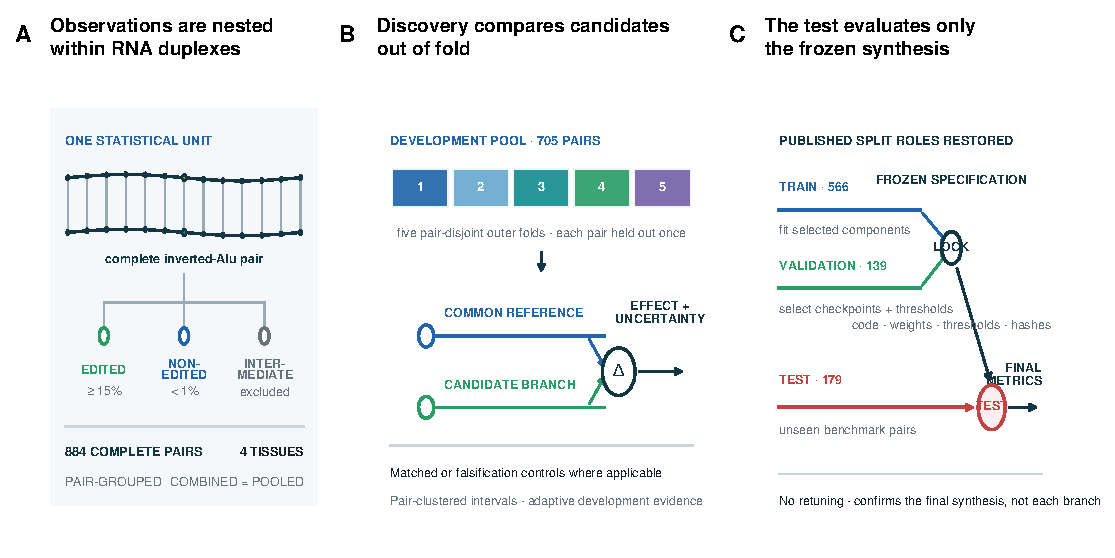
\includegraphics[width=\textwidth]{figures/figure1_systematic_dissection.pdf}
\caption{\textbf{An information hierarchy and leakage-safe strategy for mapping endogenous editing.} (A) Intrinsic substrate properties, focal target/partner alignment, and cellular realization delimit observed editing; pair burden is an indirect readout of substrate propensity. Illustrations are conceptual. (B) Controlled comparisons interrogated context, supervision, representation, and generalization. (C) Complete pairs were partitioned globally, development used pair-disjoint folds, and the final specification was frozen before one canonical held-out evaluation. Combined is pooled and received no tissue-specific state vector.}
\label{fig:overview}
\end{figure*}

\subsection*{Sequence and predicted structure recover broad but non-universal signal}

Whole-duplex sequence and predicted structure recover substantial editing signal across tissues and lineages. In retained benchmark characterization runs, the compact sequence--structure baseline achieved within-context AUROC of 0.869--0.933 across the five human endpoints and 0.823--0.865 across three nonhuman datasets (Fig.~\ref{fig:scope}A). These values are descriptive across datasets rather than estimates of a common effect, but they establish that intrinsic RNA information is informative beyond one species or tissue.

Transfer delineated the scope of that signal. Models transferred strongly among human endpoints, whereas transfer among nonhuman datasets was more variable and human--nonhuman transfer was lower and asymmetric (Fig.~\ref{fig:scope}B and C). The results support a shared but non-universal sequence--structure grammar; the present datasets cannot separate contributions from lineage, substrate composition, assay, and cellular environment.

High discrimination does not imply biological completeness. A sequence--structure model can rank sites while leaving substrate availability, tissue state, and unmeasured conformations unresolved. Subsequent tests therefore measured information added beyond this baseline rather than treating accuracy as variance explained.

\begin{figure*}[t!]
\centering
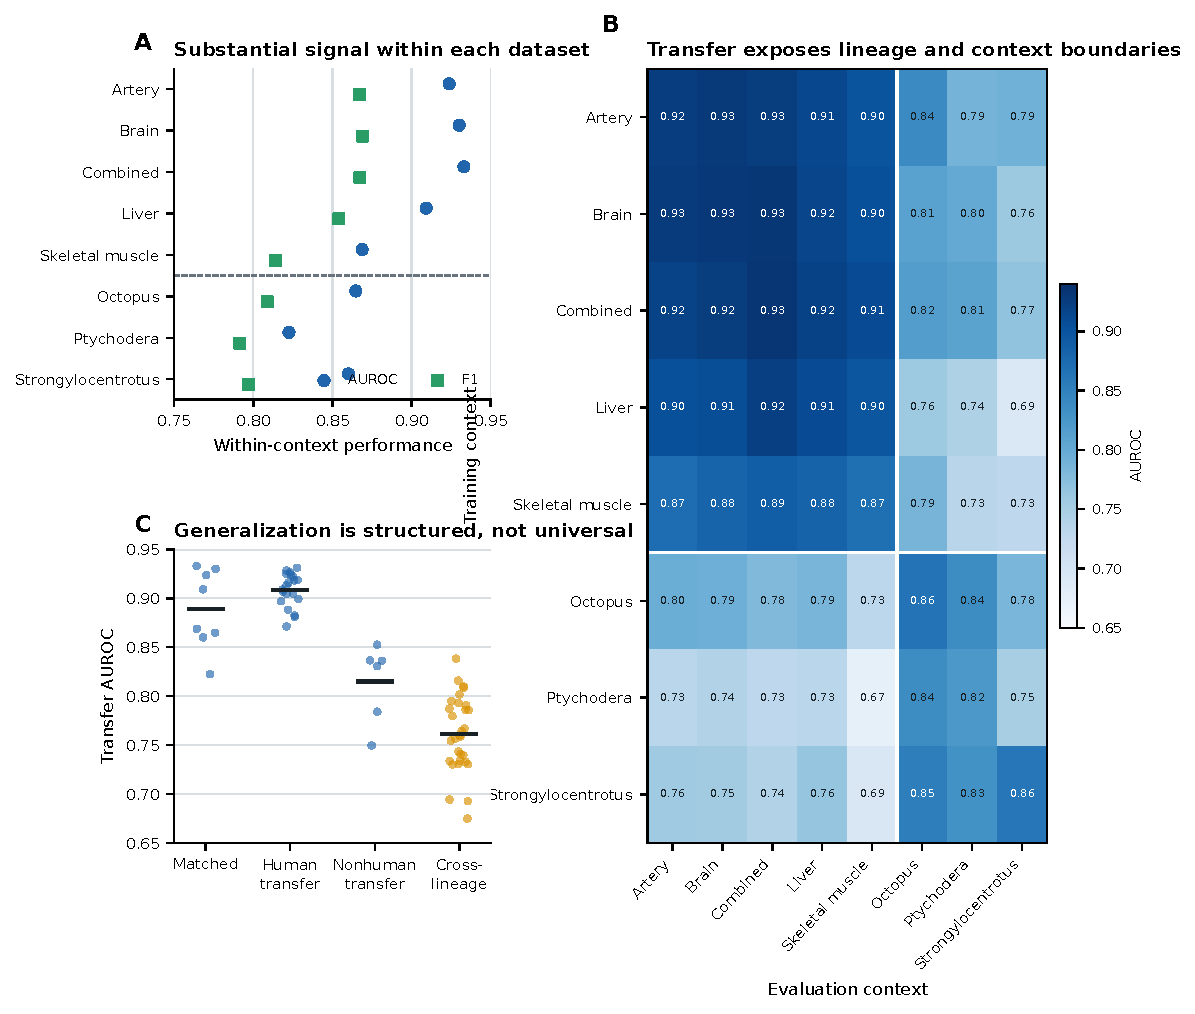
\includegraphics[width=\textwidth]{figures/figure2_sequence_scope.pdf}
\caption{\textbf{Sequence--structure information is substantial but not universal.} The tissue and lineage illustrations identify dataset classes and encode no measured values. (A) Within-context AUROC and F1 for the retained compact sequence--structure baseline across five human endpoints and three nonhuman datasets. Combined is pooled. (B) AUROC when each training context is evaluated in every context; white lines separate human and nonhuman blocks, and outlined diagonal cells mark matched-context evaluations. (C) Transfer values grouped by relation between training and evaluation contexts; horizontal bars are group means. These heterogeneous datasets define predictive scope but do not support causal attribution or meta-analysis.}
\label{fig:scope}
\end{figure*}

\subsection*{Substrate organization reveals an editing-propensity layer}

Substrate organization carries information about editing burden that the RNA graph does not encode. Genomic separation between Alu arms---discarded when model inputs join them with a fixed separator---correlated negatively with edited-site fraction in every individual tissue (Spearman $\rho=\MuscleGapRho{}$ to $\ArteryGapRho{}$; Fig.~\ref{fig:evidence}B). Low-capacity models combining geometry with graph summaries predicted pair-level edited fraction with $R^2=\MuscleEngagementCombinedGeometryRSquared{}$--\LiverEngagementCombinedGeometryRSquared{} and outperformed graph summaries alone in every tissue (Fig.~\ref{fig:evidence}C; SI Appendix). Pair geometry therefore marks a reproducible substrate-level propensity, although it does not directly measure duplex realization or ADAR engagement.

\begin{figure*}[t!]
\centering
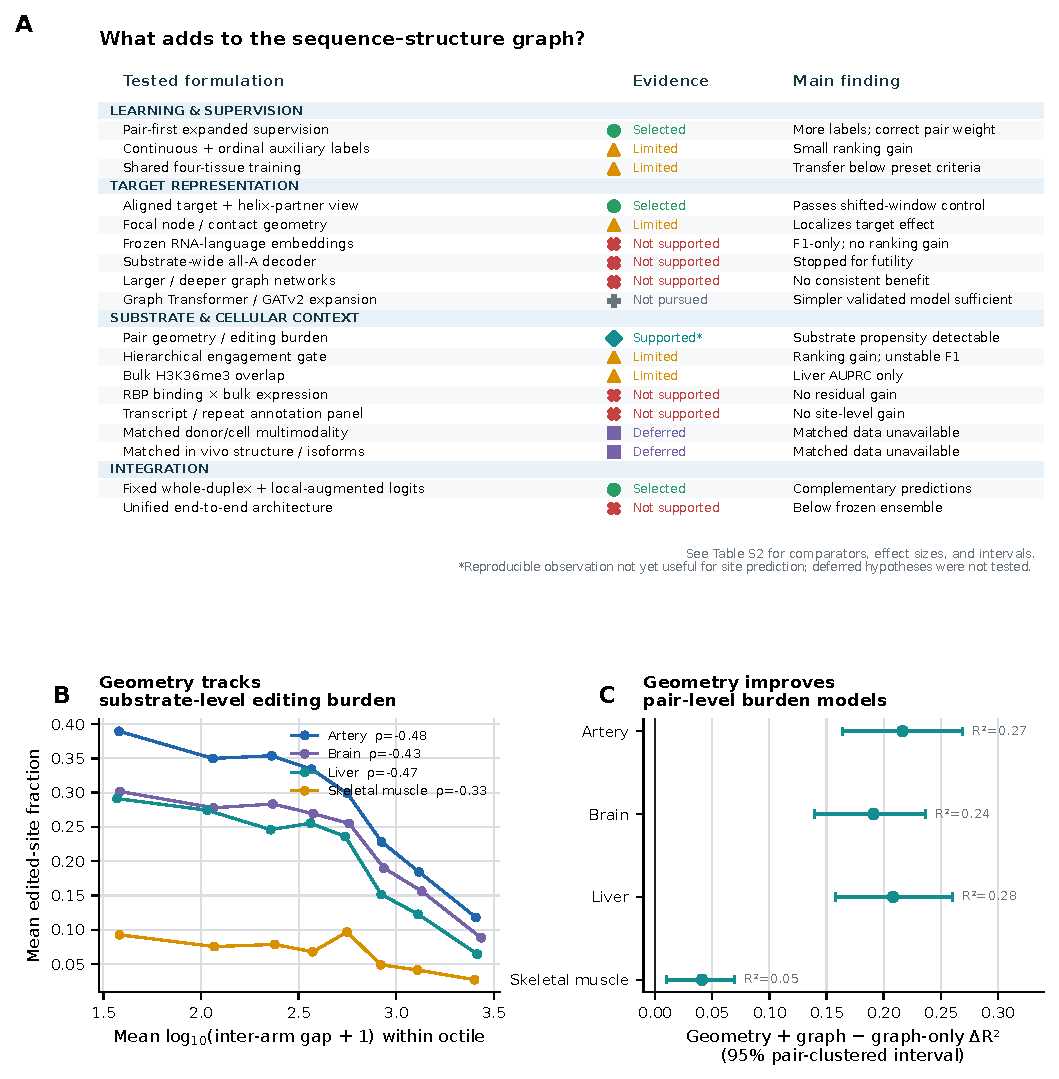
\includegraphics[width=0.98\textwidth]{figures/figure2_evidence_map.pdf}
\caption{\textbf{A substrate-level signal remains unresolved by current context measurements.} (A) Tested information sources grouped by scale and outcome; the left hierarchy maps directly to the evidence sections. SI Appendix, Table S2 gives each comparator, effect size, and interval. ``Supported$\dagger$'' denotes a reproducible substrate-level observation not yet useful for site prediction; ``not supported'' applies only to the tested formulation, and deferred measurements were unavailable. (B) Mean edited-site fraction across octiles of inter-arm gap in four tissues; $\rho$ is calculated over individual development pairs. (C) Increment in pair-level $R^2$ from adding genomic geometry to graph summaries. Bars are 95\% pair-clustered bootstrap intervals; labels give absolute $R^2$ for the combined model.}
\label{fig:evidence}
\end{figure*}

\subsection*{Current bulk measurements do not resolve the latent cellular state}

Available bulk annotations did not recover the state that converts substrate propensity into reliable site-level predictions. A cross-fitted engagement gate added \EngagementGateDeltaAUPRCMedian{} AUPRC but only \EngagementGateDeltaFOneMedian{} F1, whose interval included zero, and increased Brier score by \EngagementGateDeltaBrierMedian{}. A neural engagement auxiliary likewise failed its prespecified criterion. Static geometry marks a stable propensity, but cannot reveal whether a particular transcript formed the expected duplex, remained accessible, occupied the right compartment, or encountered active ADAR.

The initial cellular-context hypothesis focused on RBP competition. We tested replicated ENCODE eCLIP occupancy, sequence-based RBP predictions, tissue abundance, binding-by-abundance interactions, literature-prioritized regulators, and randomized or shuffled controls \cite{VanNostrand2020,Sun2021PrismNet,Horlacher2023RBPNet,GTEx2020}. Sequence-based predictions complemented eCLIP, for which Alu multimapping makes peak absence ambiguous. Neither cell-line occupancy nor tissue-average abundance contributed reproducible residual information. Cross-tissue label switches were also nearly separated by tissue identity alone, preventing four tissue means from identifying an RBP-specific transferable effect. Bulk and cell-line proxies therefore did not resolve transcript-specific regulator exposure; matched cell- or donor-level assays are the more informative next test \cite{Freund2020,QuinonesValdez2019,Park2026,Yi2026}.

Broad transcript, repeat-subfamily, divergence, and neighborhood annotations likewise failed to improve site-level prediction beyond the graph. Exact-tissue bulk H3K36me3 overlap produced a small liver AUPRC increment without stable AUROC, F1, or pair-level benefit. This weak effect points toward quantitative, sample-matched assays of cotranscriptional state rather than binary tissue-level overlap \cite{Cai2026,ENCODE2020}. Together, these results sharpen the measurement problem: substrate-level propensity is detectable, but available static and tissue-average proxies do not resolve the cellular state needed to improve the strongest site classifier.

\subsection*{The RNA duplex is the effective statistical unit}

Treating the duplex as the sampling unit improves prediction independently of adding labels. The canonical row set samples only part of the available high- and low-editing observations, and uniform site sampling gives each substrate influence proportional to its number of observations. Yet sites within one duplex share sequence, structure, genomic context, and often editing behavior; they are not independent biological units.

A same-fold ablation separated label recovery from pair weighting in muscle (Fig.~\ref{fig:principles}A; SI Appendix). Adding all high/low observations under row-wise sampling improved AUROC by \MuscleLabelExpansionAUROCMedian{} percentage points (95\% pair-clustered interval \MuscleLabelExpansionAUROCLower{} to \MuscleLabelExpansionAUROCUpper{}) and F1 by \MuscleLabelExpansionFOneMedian{} points (\MuscleLabelExpansionFOneLower{} to \MuscleLabelExpansionFOneUpper{}). Holding that expanded pool fixed and drawing a pair before class and site contributed a further \MusclePairFirstIncrementAUROCMedian{} AUROC points (\MusclePairFirstIncrementAUROCLower{} to \MusclePairFirstIncrementAUROCUpper{}) and \MusclePairFirstIncrementFOneMedian{} F1 points (\MusclePairFirstIncrementFOneLower{} to \MusclePairFirstIncrementFOneUpper{}). Thus label recovery and substrate weighting make separable contributions.

The pair-first formulation improved the same-fold reference in all five endpoints (Fig.~\ref{fig:principles}B); all 15 AUROC, AUPRC, and F1 intervals excluded zero. The duplex, rather than an arbitrarily abundant set of its rows, is therefore the effective unit for weighting observations during learning.

\subsection*{Target alignment recovers site-level predictive information}

Preserving the focal adenosine and its predicted helix partner recovers site-level information diluted by whole-duplex pooling. Simple target-contact geometry improved ranking and calibration but not F1, and explicitly retaining the focal graph node improved AUROC and AUPRC more consistently than an otherwise matched duplicate-global control. Both results localized predictive information near the target before a specialized local encoder was built.

The selected local-augmented graph predictor adds a \LocalWindowWidth{}-position representation centered jointly on the focal adenosine and its dot-bracket-aligned helix partner. A low-capacity dilated convolution encodes nucleotide identity, pairing state, focal and partner indicators, and signed relative position; its output is fused with the whole-duplex graph embedding before classification. In muscle OOF data it reached AUROC/AUPRC/F1 of \MuscleLocalAUROC{}/\MuscleLocalAUPRC{}/\MuscleLocalFOne{}, compared with \MusclePairAUROC{}/\MusclePairAUPRC{}/\MusclePairFOne{} for the pair-first whole-duplex-only predictor (Fig.~\ref{fig:principles}C).

The decisive control retained the same graph-plus-convolution architecture and optimization but shifted the local center by \LocalControlShift{} nt. Performance fell to \MuscleShiftedAUROC{}/\MuscleShiftedAUPRC{}/\MuscleShiftedFOne{}. Aligned-minus-shifted differences were \AlignedMinusShiftedAUROCMedian{} AUROC, \AlignedMinusShiftedAUPRCMedian{} AUPRC, and \AlignedMinusShiftedFOneMedian{} F1, with entirely positive pair-clustered intervals. This matched-capacity shift sharply reduced performance, localizing the gain to target alignment rather than added convolutional capacity. Liver replication and the secondary natural-prevalence analysis showed the same pattern.

\subsection*{Whole-duplex and target-local information remain complementary}

The local-augmented predictor did not make an independently optimized whole-duplex view redundant. Their errors remained sufficiently distinct that a fixed mean of logits improved the whole-duplex-only predictor by \MuscleEnsembleDeltaAUROCMedian{}/\MuscleEnsembleDeltaAUPRCMedian{}/\MuscleEnsembleDeltaFOneMedian{} AUROC/AUPRC/F1 in muscle and \LiverEnsembleDeltaAUROCMedian{}/\LiverEnsembleDeltaAUPRCMedian{}/\LiverEnsembleDeltaFOneMedian{} in liver; all six pair-clustered intervals excluded zero (Fig.~\ref{fig:principles}D).

The final predictive specification consequently used two independently trained pair-first components: a whole-duplex-only graph predictor and a second graph predictor internally augmented with the aligned target/helix-partner convolution. Their logits are combined by a fixed \EnsembleComponentWeight{}/\EnsembleComponentWeight{} mean; the weights were not searched (Fig.~\ref{fig:principles}E). Fixed integration preserved complementary predictive views without fitting a flexible stacker to only hundreds of independent substrates.

\begin{figure*}[t!]
\centering
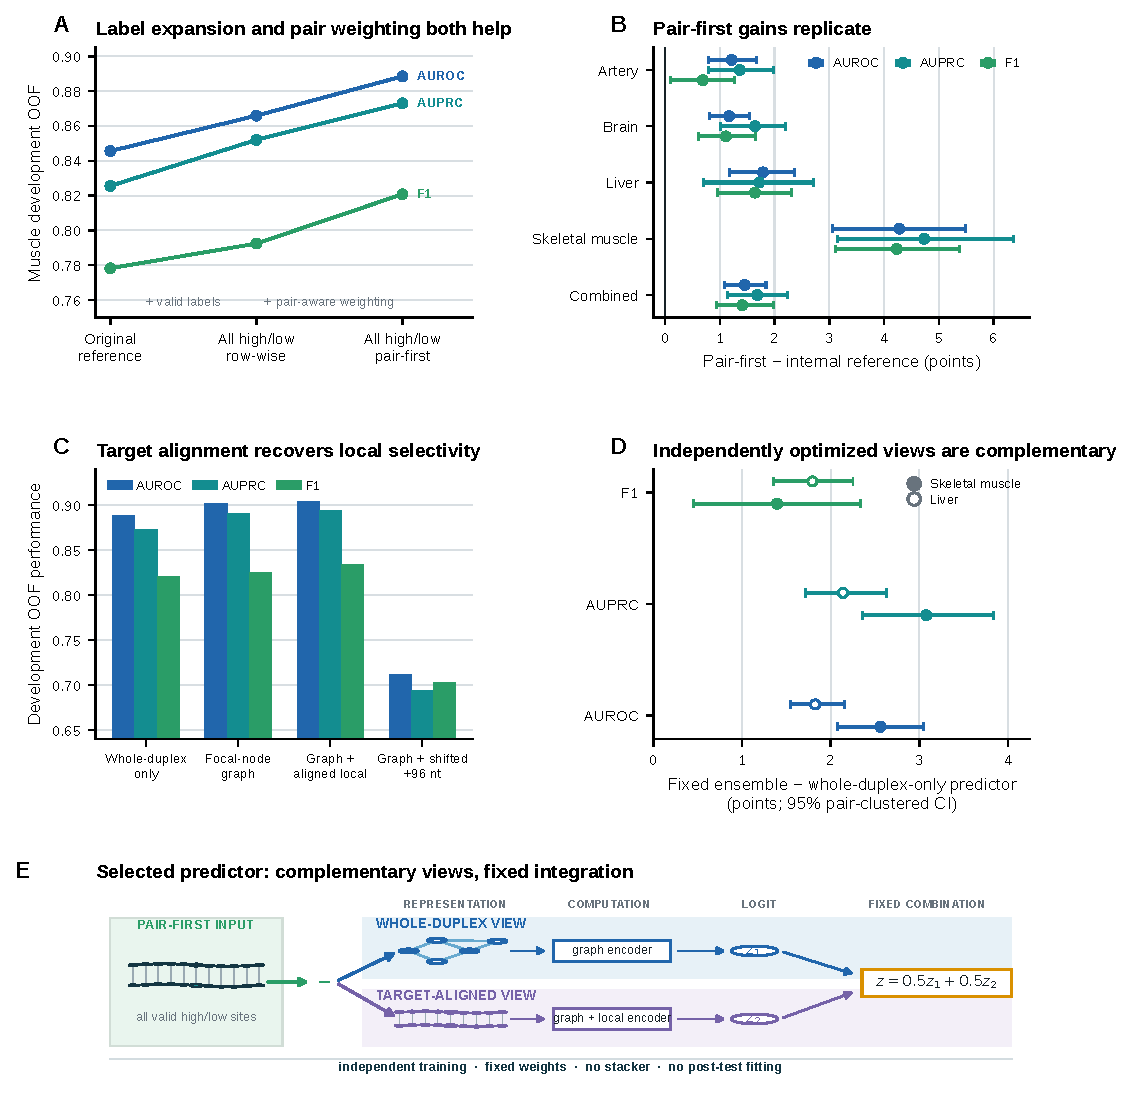
\includegraphics[width=\textwidth]{figures/figure3_organizing_principles.pdf}
\caption{\textbf{Substrate-aware learning and target alignment recover complementary information.} (A) Same-fold ablations separate recovery of additional valid high/low labels from pair-first weighting. (B) Pair-first expanded supervision improves the internal reference across all five endpoints; points and bars are pair-clustered medians and 95\% intervals. (C) Whole-duplex pooling, focal-state retention, and aligned-local fusion form an evidence ladder; an otherwise identical local model shifted by \LocalControlShift{} nt fails. (D) A fixed equal-logit ensemble improves its whole-duplex-only component in muscle and liver. (E) The operational predictor combines independently trained whole-duplex-only and graph-plus-local models without searched weights or post-test fitting. The RNA illustration is conceptual. All panels show development evidence.}
\label{fig:principles}
\end{figure*}

\subsection*{Richer supervision and model complexity yield diminishing returns}

Once substrate-aware sampling and target alignment were in place, richer supervision and cross-tissue sharing produced only small ranking gains. Binary/ordinal/continuous learning and a shared four-tissue encoder both fell below their predeclared selection criteria, and each introduced an adverse tradeoff in thresholded performance or calibration. These results show that graded labels and shared contexts contain some information, but substantially less than correcting the sampling unit and preserving target position (Fig.~\ref{fig:evidence}A; SI Appendix).

Generic increases in representation or capacity likewise failed to move the boundary. A substrate-wide all-adenosine decoder met its prespecified futility criterion; frozen RiNALMo embeddings added no control-robust ranking gain; and larger graph networks were not consistently better \cite{Penic2025}. A preregistered connected model combining the successful global, focal, and aligned-local views then underperformed the frozen prediction-level ensemble in AUROC and AUPRC in every fold and worsened Brier score (SI Appendix). Thus, performance saturated when added inputs did not match the biological scale of the missing information. This boundary is conditional on the tested measurements, representations, and effective sample size.

\subsection*{A frozen predictor validates the selected principles on the untouched benchmark}

After development selection, the complete predictor---components, checkpoints, thresholds, weights, code, and hashes---was frozen before one authorized evaluation on the canonical test.

The resulting predictor, ADARPro, improved AUROC, AUPRC, and F1 in all five reported endpoints (Fig.~\ref{fig:locked}A), with mean gains of \MacroDeltaAUROC{}, \MacroDeltaAUPRC{}, and \MacroDeltaFOne{} over reproduced supplied-checkpoint AdarEdit. Every endpoint had a positive 95\% pair-clustered interval for all three metrics, and Brier score decreased throughout (Fig.~\ref{fig:locked}B and C; SI Appendix, Table S1). Combined overlaps the individual tissue endpoints, so the mean is descriptive rather than a five-tissue meta-analysis. The canonical result confirms that substrate-aware learning and target alignment carry information beyond the published predictor.

The gains were not purchased by indiscriminate suppression of positive calls. At frozen validation-selected thresholds, ADARPro corrected \CombinedFPRescueRate{}--\LiverFPRescueRate{}\% of baseline false positives while damaging \CombinedTPDamageRate{}--\LiverTPDamageRate{}\% of baseline true positives (Fig.~\ref{fig:locked}D). A secondary matched-recall analysis is reported in SI Appendix, Table S9.

\begin{figure*}[t!]
\centering
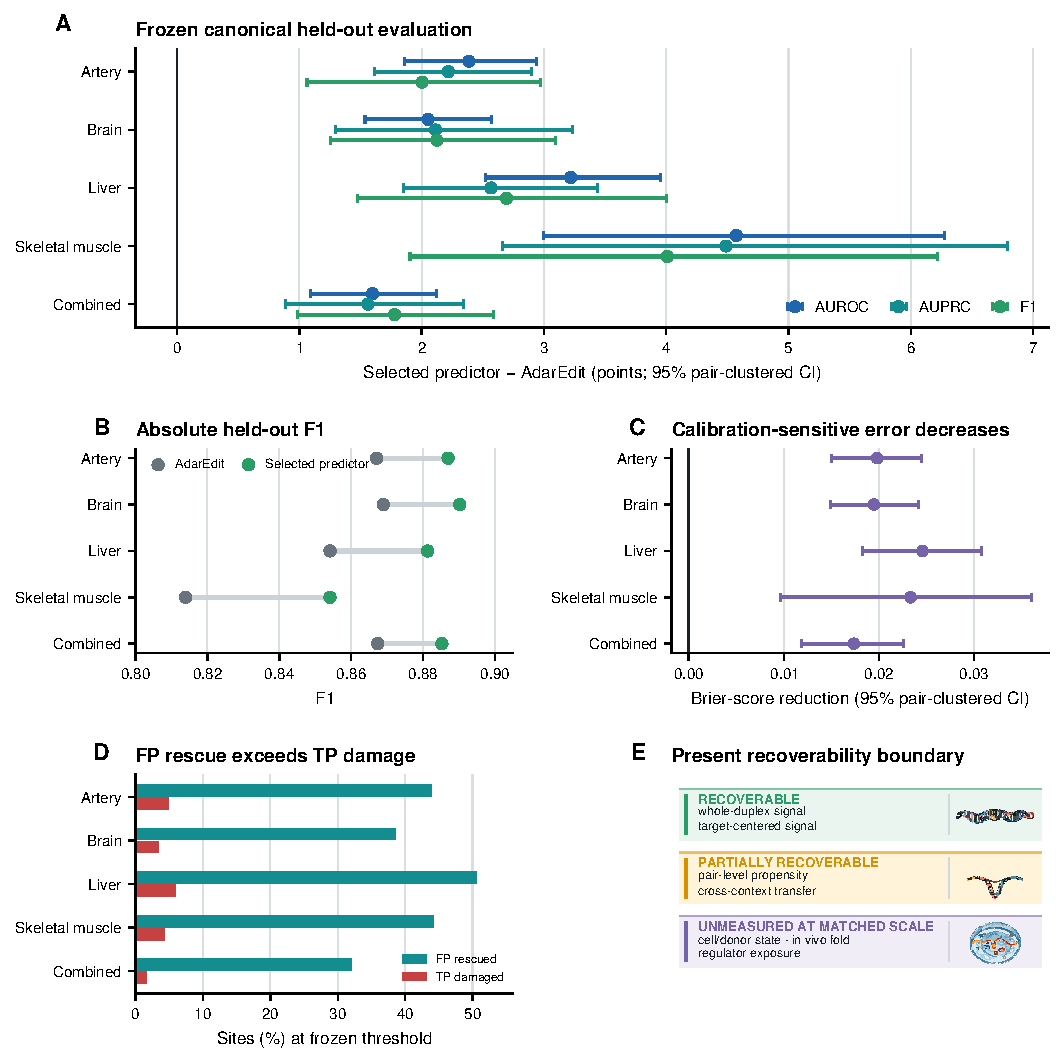
\includegraphics[width=\textwidth]{figures/figure4_locked_validation.pdf}
\caption{\textbf{Frozen validation confirms the selected principles and summarizes the present boundary.} (A) ADARPro minus reproduced supplied-checkpoint AdarEdit for AUROC, AUPRC, and F1; bars are 95\% pair-clustered bootstrap intervals. (B) Absolute F1. (C) Reduction in Brier score. (D) Baseline false positives corrected and baseline true positives damaged at frozen validation-selected thresholds. (E) Information captured, partially resolved, and missing at a matched biological scale; tier-specific icons are conceptual. Combined is pooled. All quantitative panels use the single-use canonical held-out evaluation.}
\label{fig:locked}
\end{figure*}

\section*{Discussion}

Endogenous A-to-I editing contains distinct predictive information at the substrate and nucleotide scales. Whole-duplex sequence and predicted structure encode broadly transferable intrinsic suitability; genomic organization marks a reproducible substrate-level editing propensity; and target/helix-partner alignment recovers local information obscured by whole-duplex pooling. Pair-first learning adds a statistical principle: correlated sites from one duplex must not acquire influence simply because that substrate contributes more rows.

This map connects observations that prior studies often treated separately. Sequence preferences and helix context are established determinants of local editability, whereas the distance between oppositely oriented Alus predicts aggregate Alu editing \cite{Eggington2011,Bazak2014Editability,ZambranoMila2023}. Perturbational studies further establish regulation by RBPs and chromatin-associated processes \cite{Freund2020,QuinonesValdez2019,Cai2026,Park2026,Yi2026}. Our results place these findings on different information scales: intrinsic RNA and target context are recoverable from the benchmark, but cell-line occupancy and tissue-average abundance or chromatin do not identify regulator exposure or substrate state on an individual transcript. Their failure here reflects measurement resolution, not absence of the underlying biology.

The remaining boundary is empirical. Once whole-duplex and aligned target information were represented and substrate dependence was respected, graded labels, shared training, generic RNA embeddings, larger graph capacity, and joint end-to-end integration produced diminishing or adverse returns. Residual error may reflect donor- or cell-specific ADAR abundance and isoform state, interferon response, transcript processing, regulator occupancy, in vivo conformation, measurement error, finite data, representation limits, or biological stochasticity; these experiments cannot apportion those sources. The unresolved quantity is therefore not a single hidden mechanism, but transcript- and cell-resolved state absent from the current benchmark.

Several limitations define the scope of this conclusion. The primary benchmark comprises graph-buildable human inverted-Alu substrates and tissue summaries, not all editing substrates or donor-resolved measurements. The nonhuman datasets differ in lineage, substrate class, and data generation, so they reveal transfer limits without identifying their cause. Predicted secondary structure is only a surrogate for conformations available to ADAR in vivo. The canonical task is balanced and excludes intermediate observations; natural-prevalence analyses are secondary. eCLIP coverage is cell-line-specific and compromised by repeat mapping. Finally, an independent cohort is needed to test transportability beyond the existing benchmark construction.

The frozen predictor validates the practical value of the information map: substrate-aware supervision and target-centered representation improve held-out discrimination, classification, and calibration. The broader result is a measurement agenda. Editing, transcript abundance and processing, splicing and intron retention, ADAR isoform and interferon state, enzyme activity and localization, regulator occupancy, quantitative chromatin, and in vivo RNA conformation must be measured in the same donors or cells and on the same substrates. Such data could test whether cellular state governs realization of a suitable duplex while local RNA context governs selection of particular adenosines.

\matmethods{
\subsection*{Benchmark and labels}
We used the AdarEdit v2 reproducibility release at upstream revision \texttt{5c8b57d70cdc2eb1c5e168431013275bcc9ed0c5}. The benchmark contains \NSubstrates{} graph-buildable inverted-Alu pairs. Human labels were edited for EditingIndex $\geq\PositiveThresholdPct{}\%$, nonedited for EditingIndex $<\NegativeThresholdPct{}\%$, and intermediate otherwise. The canonical task excludes intermediate observations. Pair identities and the fixed \NTrainPairs{}/\NValidationPairs{}/\NTestPairs{} train/validation/test assignment were verified before analysis. Combined was treated only as its published pooled endpoint.

\subsection*{Development protocol}
All discovery used the original train plus validation pairs divided into \NOuterFolds{} outer folds by pair ID. Learned preprocessing, feature selection, checkpoint choice, and threshold choice were fitted without the outer fold. Predictions were concatenated only after every row was scored by a model that had not trained on its pair. The test paths were protected by a stateful quarantine. Development OOF metrics estimate same-fold incremental effects; supplied-checkpoint test metrics remain the authoritative reference.

\subsection*{Models}
The first component retained the compact AdarEdit graph attention encoder and trained from the expanded high/low site pool using uniform pair-first and equal-class sampling. The second, independently trained component retained the same graph encoder and added a \LocalWindowWidth{}-position target/helix-partner-aligned representation encoded by two dilated convolutional layers; local and graph embeddings were fused before its prediction head. The selected probability was $\sigma[(\operatorname{logit}p_{\mathrm{whole}}+\operatorname{logit}p_{\mathrm{augmented}})/2]$; weights were fixed at \EnsembleComponentWeight{}/\EnsembleComponentWeight{} rather than searched. The shifted-window control preserved the graph-plus-convolution architecture and optimization while moving the local center \LocalControlShift{} nt. Full feature definitions, architectures, ablations, and biological-context protocols are in SI Appendix.

\subsection*{Statistics and final evaluation}
Metrics were AUROC, AUPRC, F1, precision, recall, specificity, balanced accuracy, MCC, and Brier score. Thresholds maximized validation F1 within each frozen training run. Uncertainty used a pair-clustered bootstrap with \NBootstrapReplicates{} replicates that resampled Alu pairs and retained all their sites. Development intervals quantify paired effect uncertainty and were not treated as multiplicity-adjusted confirmatory tests; selection also required recorded decision criteria and controls. Before final evaluation, code, inputs, weights, epochs, thresholds, and checkpoint SHA-256 values were frozen. Test authorization was consumed once, and no post-test model selection or tuning occurred. Natural-prevalence and matched-recall analyses are secondary and described in SI Appendix.

}

\showmatmethods{}

\dataavail{Code, experiment configurations, registries, source tables, figure scripts, retained derived artifacts, frozen checkpoints, and provenance are available at \url{https://github.com/Scientific-Computing-Lab/ADARPro}. Third-party downloads and deterministic matrices omitted from GitHub are listed with source URLs, roles, checksums, and regeneration instructions in the data manifest. GPT Image 1.5 generated only label-free, nonquantitative figure components; prompts, candidate selection, and hashes are disclosed in the repository. The AdarEdit benchmark is available from \url{https://github.com/Scientific-Computing-Lab/AdarEdit}. No new human participants were recruited and no new primary sequencing data were generated.}

\acknow{Acknowledgments and funding information pending author confirmation.}
\showacknow{}

\bibsplit[15]
\bibliography{references}

\end{document}
